\documentclass[conference]{IEEEtran}
\IEEEoverridecommandlockouts
% The preceding line is only needed to identify funding in the first footnote. If that is unneeded, please comment it out.
\usepackage{cite}
\usepackage{amsmath,amssymb,amsfonts}
\usepackage{algorithmic}
\usepackage{graphicx}
\usepackage{textcomp}
\usepackage{xcolor}
\def\BibTeX{{\rm B\kern-.05em{\sc i\kern-.025em b}\kern-.08em
    T\kern-.1667em\lower.7ex\hbox{E}\kern-.125emX}}
\begin{document}

\title{Effects of HRTF on video games performance\\}

\author{\IEEEauthorblockN{Giovanni Cocco}
\IEEEauthorblockA{\textit{Computer Science Department} \\
\textit{Università degli Studi di Milano}\\
Milano, Italy \\
giovanni.cocco3@studenti.unimi.it}
}

\maketitle

\begin{abstract}
Sound clues are an important aspect in video games; the ability to localize a sound source spatially can give an advantage to players especially in action games such as FPS. Traditionally, video games spatialize sound using stereo panning, but new technologies such as HRTF can lead to better sound localization. In this paper we analyze the impact of Steam Audio implementation of HRTF with respect to stereo panning and mono audio on the performance of players. We also explore the impact of the technology on different types of sound such as white noise, step sound and shot sounds.
We found that HRTF improve player performance over stereo panning, but regarding the difference between different types of sound the result were inconclusive.
\end{abstract}

\begin{IEEEkeywords}
HRFT, Stereo panning, Video games, Performance
\end{IEEEkeywords}

\section{Introduction}
The ability to tell the direction of a sound is based on a series of clues the human brain is able to analyze.
The horizontal direction, or azimuth, can be mostly inferred by the ITD \textit{(Interaural Time Difference)} and the ILD \textit{(Interaural Level Difference)}.
The ITD is the delta time between the moment the sound reaches one ear and the moment it reaches the other. For instance a sound coming from the right will reach the right ear earlier than the left one. Knowing that the sound propagates at a certain speed is possible to know the angle of incidence \cite{b1}.
The ILD measures the loudness difference perceived by one ear and the other, as the more distance the sound travels the more energy it loses on the way. Also the head acts as an obstacle absorbing part of the energy of the sound.
Stereo panning is a simple method to spatialize a sound by acting on the ILD. It has been shown that accurate acoustic localization can be achieved by ILD alone \cite{b2}.
As ILD simulation is trivial to implement and not much computationally expensive it is used by many video games.
The sound is reproduced at a different loudness on the right headphone than on the left one. This allows the player to tell if a sound is coming from the right or the left.
Front back confusion can be resolved by the player movement in the environment \cite{b3}.
The vertical, or elevation, localization is based on more complex clues. The sound coming from different elevation hits the pinna in different ways. The pinna creates different notches in the frequency based on the elevation. The brain reinterprets this information to infer the position of the sound source \cite{b4}.
\begin{figure}[htbp]
\centerline{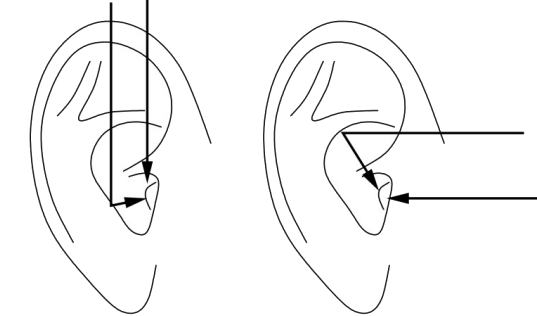
\includegraphics{pinna.png}}
\caption{Pinna effect on sounds coming from different directions}
\label{fig1}
\end{figure}
The simulation of this phenomenon is based on HRTF \textit{(Head Related Transfer Function)}.
Measurements of HRTF for some directions must first be done on a human subject or a dummy \cite{b5}.
Then it is possible to interpolate the measurements to get the missing ones \cite{b6}.
As HRTF based techniques are more computationally intensive, it is only with the improvement of computer processing power they are starting to be suitable for video games.
For this paper we used Steam Audio implementation of HRTF developed by Valve Software \cite{b7}.
As the pinna is different from one person to another so is HRTF. As such, having a personalized HRTF improves localization ability \cite{b8}. The impact of personalized HRTF based on HRTF selection was initially planned to be analyzed in this paper. HRTF selection techniques provide the user with the best matching HRTF from a database of potential HRTF. While Steam Audio allow to use custom HRTF it support only a subset of the sofa format making it not completely compatible with these methods \cite{b9}. This problem can be addressed converting the file to comply to the Steam Audio limitation. A more serious problem, which led to the drop of this part for the scope of this paper was that many HRTF datasets produced artifacts for low elevation, probably caused by a lack of measurement for these less used positions.

\section{Previous works}
Previous experiments were done on this subject.
Performance comparison between HRTF and non-HRTF based sound showed that HRTF gives better performance\cite{b10}.
Other experiments were done on the impact of HRTF individualization on VR \textit{(Virtual Reality)} games and showed that it has minimal impact with respect to generic HRTF, except for extreme elevations \cite{b11}.
Another experiment shows that the impact depends on subject sensibility and HRTF presentation order \cite{b12}.
Test was done to compare different commercial implementation of HRTF based approach may have, but found no statistically significant differences \cite{b13}. 

\section{Experiment setup}
To measure the impact on performances of different sound spatialization methods a simple video games was developed using Unity3D and Steam Audio.
In the video game the subjects were asked the shot at asteroids as fast as possible.
\subsection{Asteroids position}
Only one asteroid was present at a time in the scene.
Every time the player shot an asteroid another one instantly spawned in a random position.
The distance from the player was fixed and the asteroid was spawned in a random azimuth between 0° and 360° and a random elevation between 0° and 360°.
No check was done to disallow spawning in the player view as it was thought that it could just make the player turn as the first thing and the start thinking on how to act. The number on asteroid spawning in view should statistically be the same for each type of spatialization, balancing them out.
\begin{figure}[htbp]
\centerline{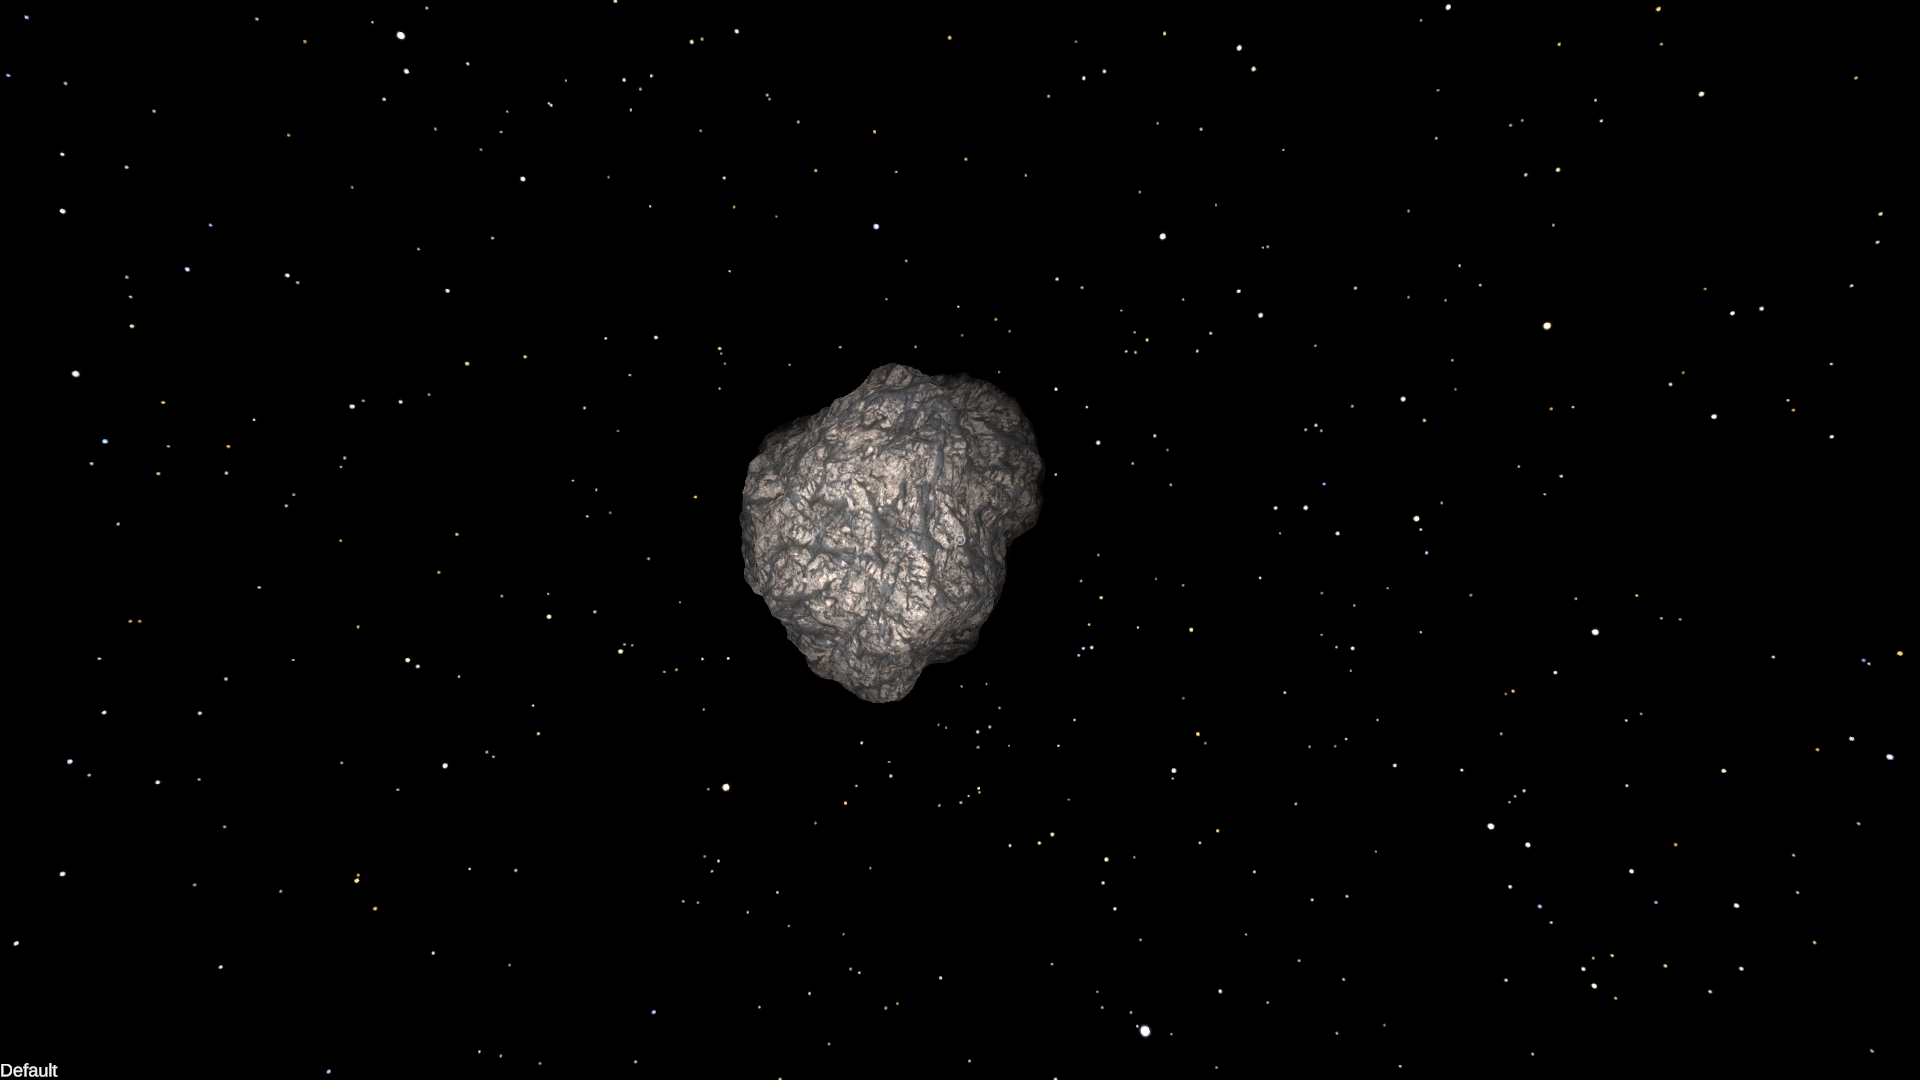
\includegraphics[scale=0.22]{gameplay.png}}
\caption{Asteroid as seen in game}
\label{fig2}
\end{figure}

\subsection{Player movement}
The player was positioned in the middle of the scene and he was not able to move spatially. The player was free to rotate the camera in both pitch and yaw with no limitation. This is not the usual FPS setup that limits pitch and does not allow a 360° rotation around that axis. This was preferred over usual FPS camera movement not to introduce any artificial movement restriction thus making the motion needed to aim to an asteroid not influenced by these potential restrictions.

\subsection{Audio clues}
The asteroids emitted sounds spatialized with different technology: mono, stereo panning and HRTF. Mono means that no sound clues are provided to the user. This was used to check if the player was simply using visual clues ignoring the audio ones. Stereo panning is the default Unity3D spatialization and provided clues on the azimuth to the player. HRTF was based on Steam Audio implementation and should provide also elevation clues.
Every asteroid had one of three possible sound types: white noise, step or shot sound. The white noise was simply a continuous white noise that should be the easier to find for the player. Step sound was a looping sound of footstep on concrete. Shot sound was a looping sound of machine gun burst with almost no pause in between bursts.

\subsection{Game session}
Each of the 21 test subjects was asked to play three game sessions, one for mono, one for stereo panning and one for Steam Audio HRTF. The session order was randomized using a Latin square to ensure that the experience a player would make in a previous session could not influence the statistical results.
In each session a total of 90 asteroids were created, 30 for each sound type: white noise, shot and step. The order was randomized ensuring the correct number of each.

\subsection{Subject setup}
The subject was asked to sit and take position at the computer with headphones on. Before each session they could freely set the volume and mouse sensibility. Mouse aim was chosen over controller because it makes possible to aim at different speed and in the experiment we wanted to check if the subjects compensates the lack of sound clues of mono increasing their speed when searching for the asteroids.

\subsection{Recorded data}
The time between when the asteroid spawned and when it got hit was recorded. Also the horizontal and vertical angular movement was recorded, i.e. the sum of the absolute values of the angles moved in each frame.

\section{Data analysis}
The collected data was analyzed using box plot and also more acurately checked with the Kolmogorov Smirnov test to see if there was any statistically significant difference between the various data collected with different audio clues or with different types of sound source.

\subsection{Box plots}
Firstly box plots were generated from the collected data.
\begin{figure}[htbp]
\centerline{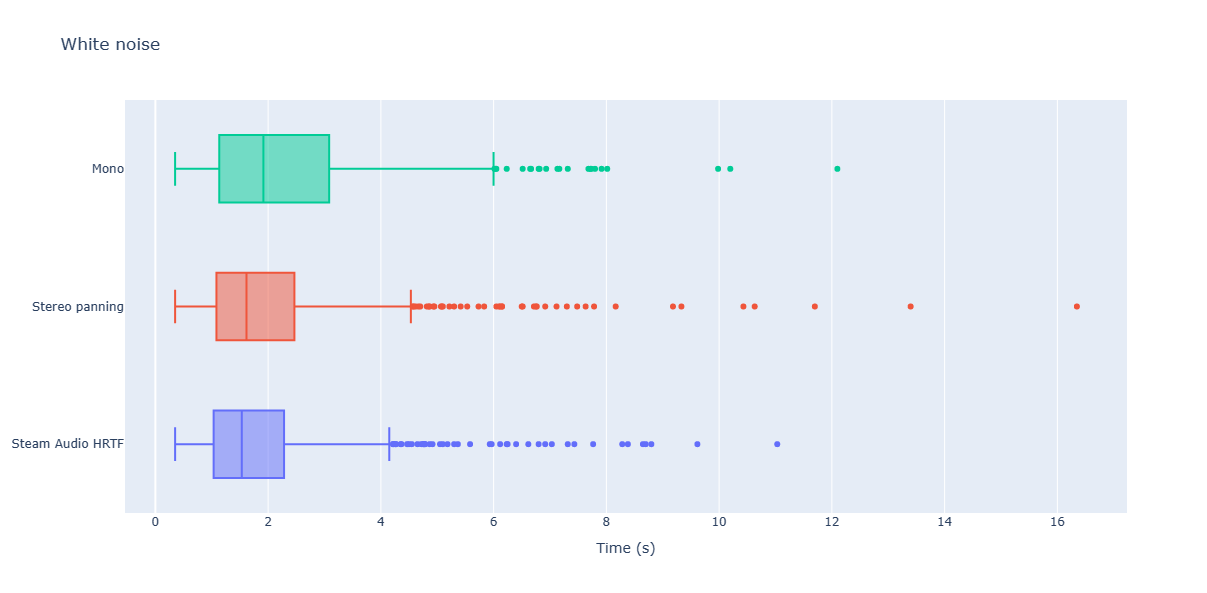
\includegraphics[scale=0.22]{white_time.png}}
\caption{Box plot of the white noise times}
\label{fig3}
\end{figure}
\begin{figure}[htbp]
\centerline{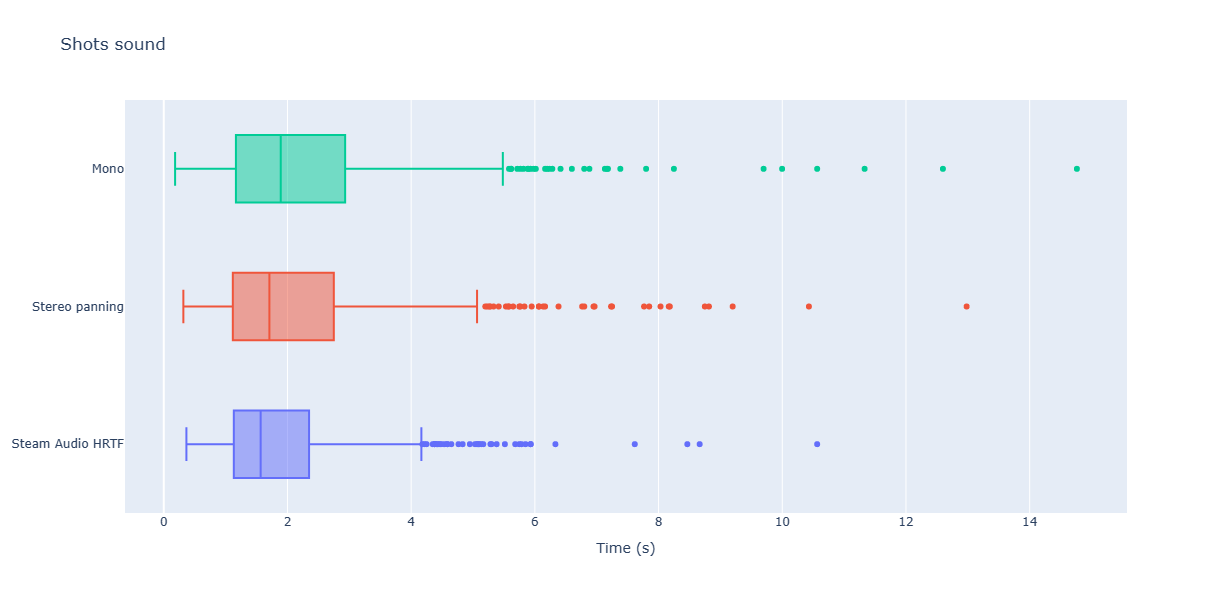
\includegraphics[scale=0.22]{shot_time.png}}
\caption{Box plot of the shot sound times}
\label{fig4}
\end{figure}
\begin{figure}[htbp]
\centerline{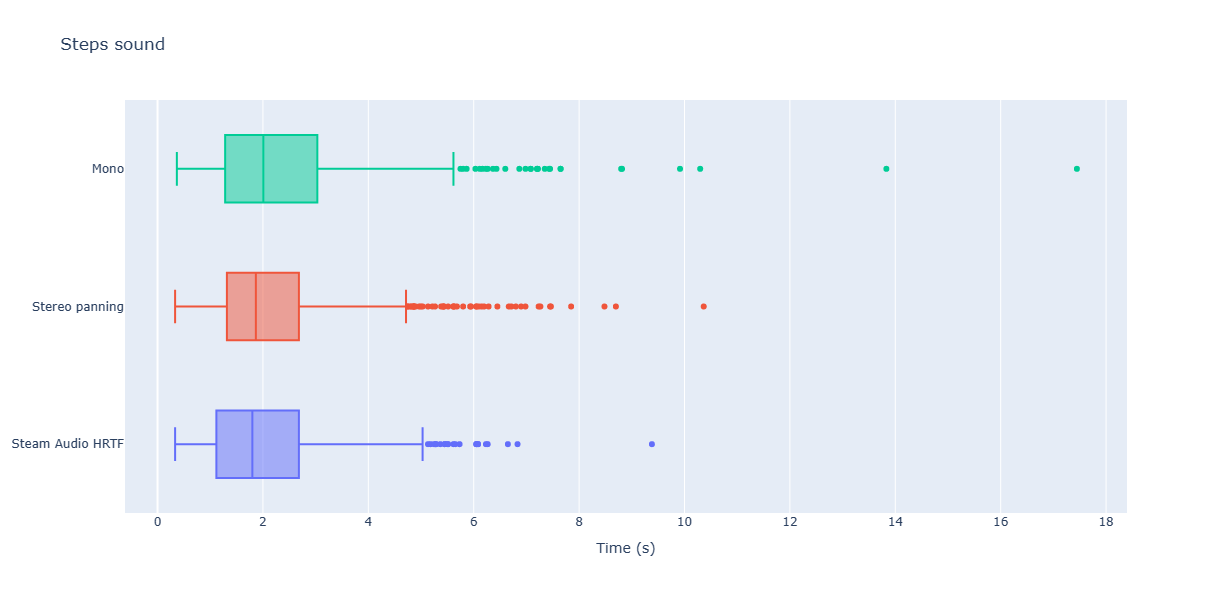
\includegraphics[scale=0.22]{step_time.png}}
\caption{Box plot of the step sound times}
\label{fig5}
\end{figure}
\begin{figure}[htbp]
\centerline{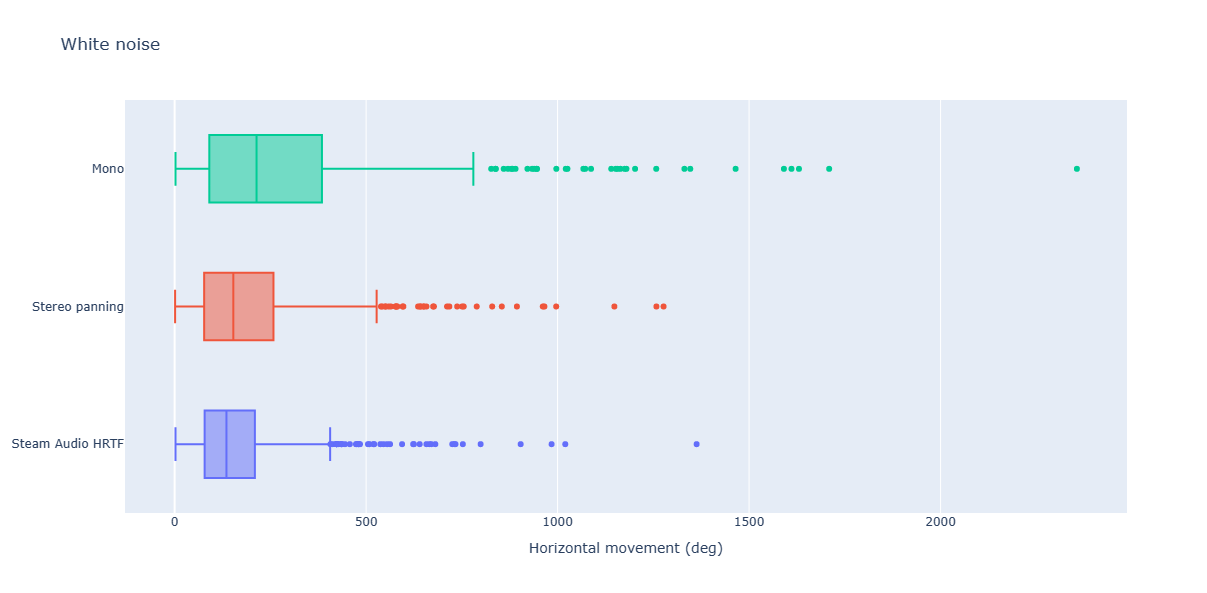
\includegraphics[scale=0.22]{white_hor.png}}
\caption{Box plot of the white noise horizontal movement}
\label{fig6}
\end{figure}
\begin{figure}[htbp]
\centerline{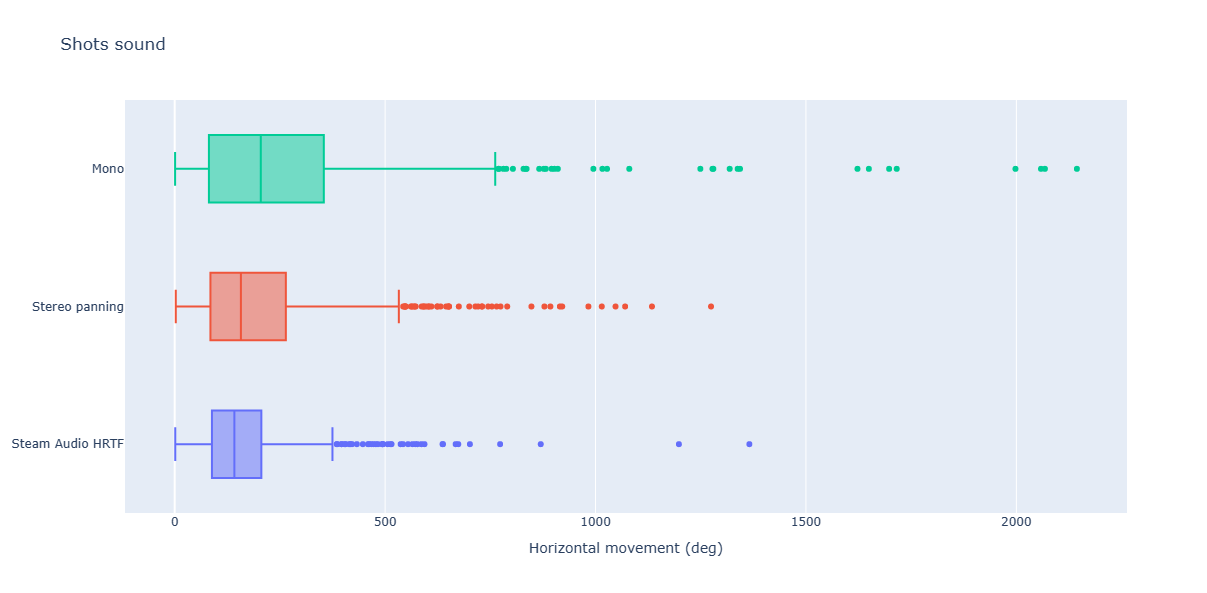
\includegraphics[scale=0.22]{shot_hor.png}}
\caption{Box plot of the shot sound horizontal movement}
\label{fig7}
\end{figure}
\begin{figure}[htbp]
\centerline{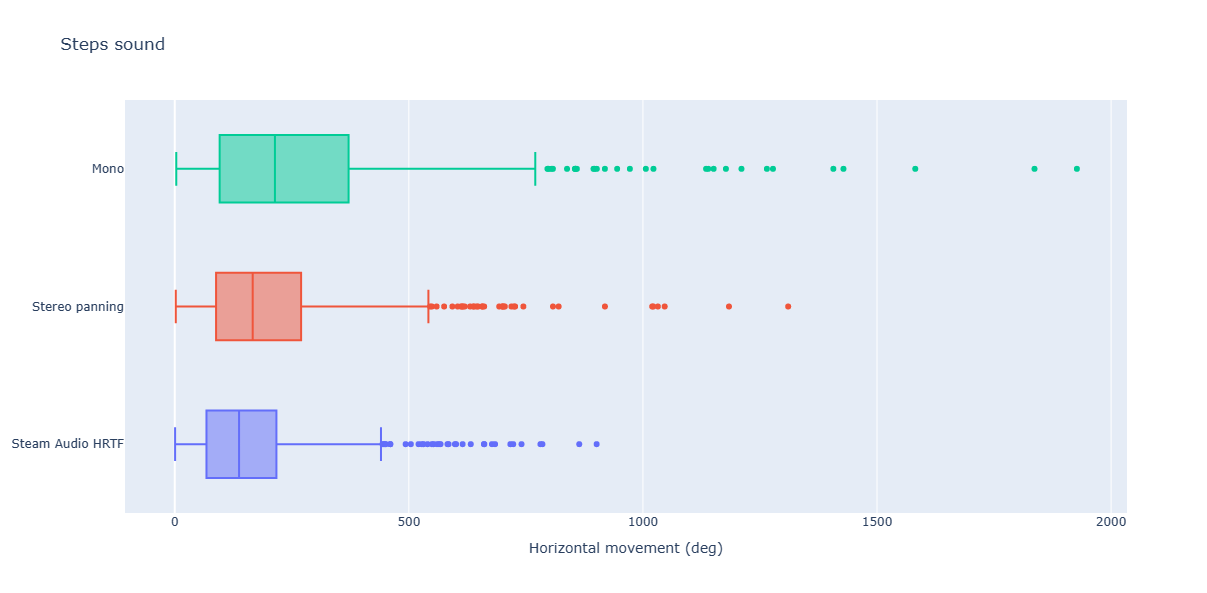
\includegraphics[scale=0.22]{step_hor.png}}
\caption{Box plot of the step sound horizontal movement}
\label{fig8}
\end{figure}
\begin{figure}[htbp]
\centerline{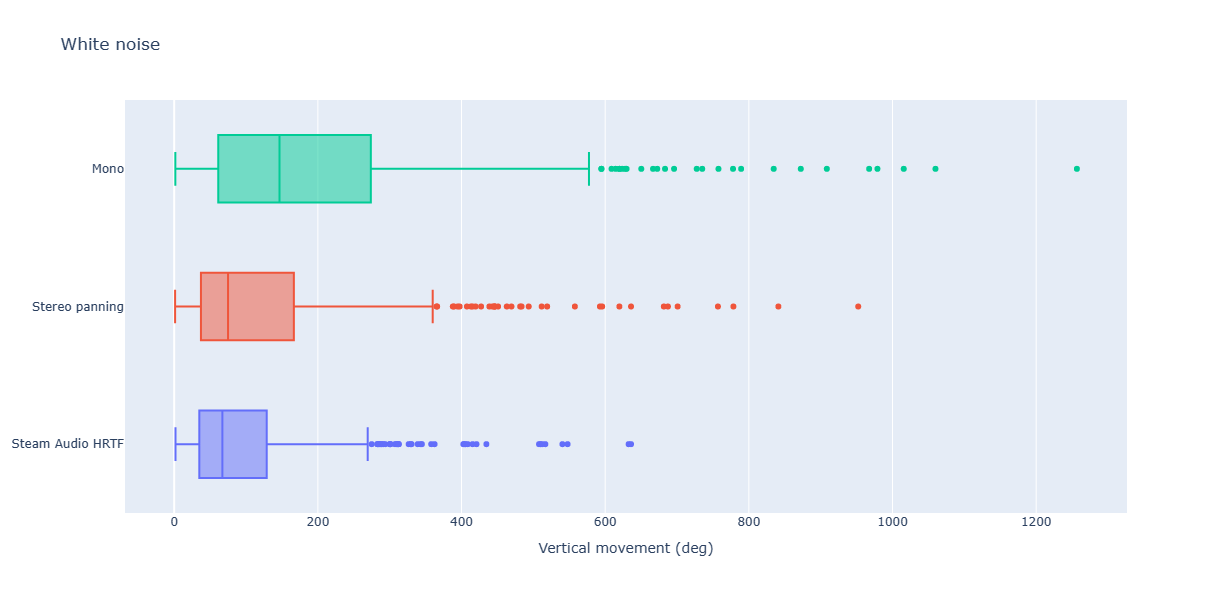
\includegraphics[scale=0.22]{white_ver.png}}
\caption{Box plot of the white noise vertical movement}
\label{fig9}
\end{figure}
\begin{figure}[htbp]
\centerline{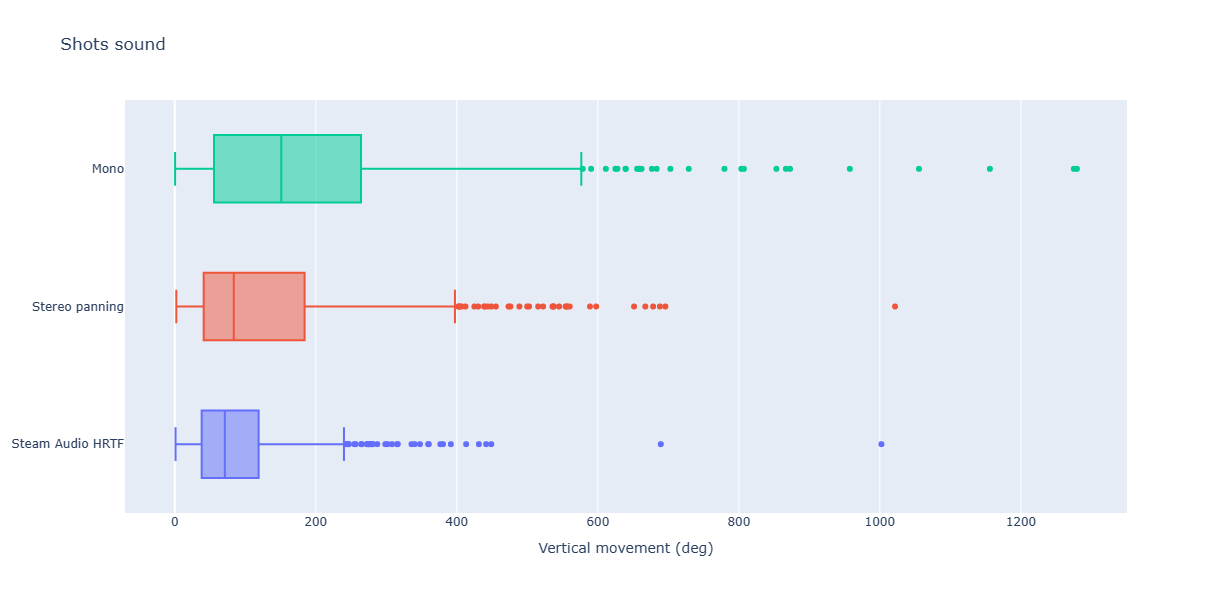
\includegraphics[scale=0.22]{shot_ver.png}}
\caption{Box plot of the shot sound vertical movement}
\label{fig10}
\end{figure}
\begin{figure}[htbp]
\centerline{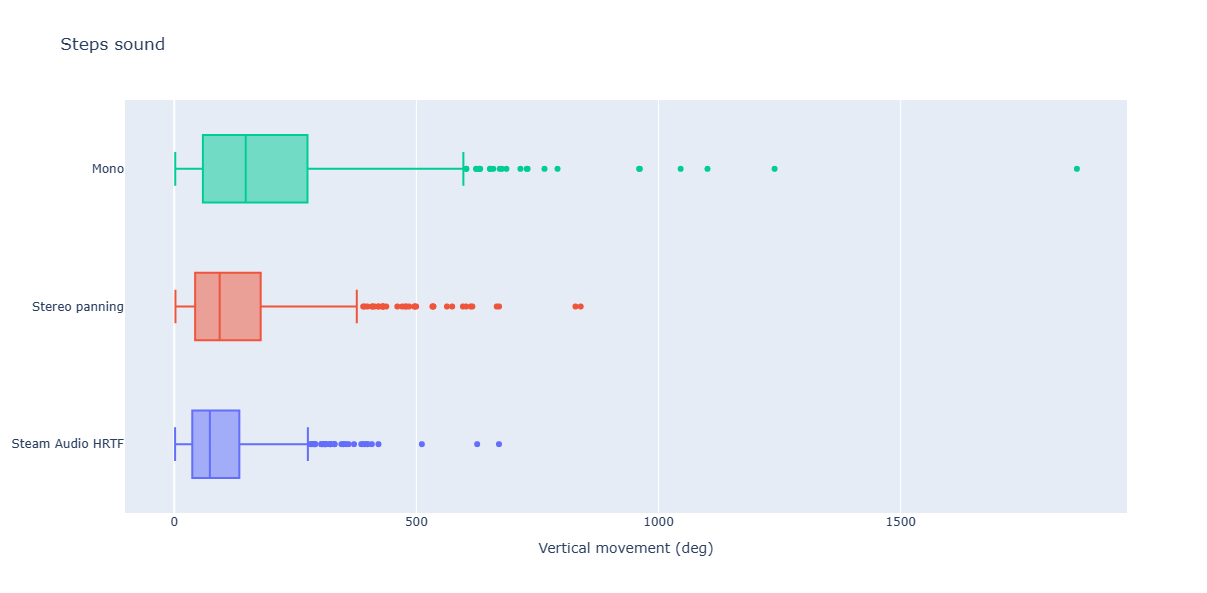
\includegraphics[scale=0.22]{step_ver.png}}
\caption{Box plot of the step sound vertical movement}
\label{fig11}
\end{figure}
\clearpage
\subsubsection{White noise times}
The analysis of the white noise times give us a median value of 1.91 seconds for mono, 1.61 seconds for stereo panning and 1.53 seconds for Steam Audio HRTF. This, as expected, suggests that giving audio clues to subjects improve the time (as mono is the worst one). It also shows how HRTF improve performance with respect to the more classic stereo panning approach.\\

\subsubsection{Shot sounds times}
Gunshot times give us a median value of 1.89 seconds for mono audio, 1.71 seconds for stereo panning and 1.57 for Steam Audio HRTF. These values are somewhat similar to the previous ones. The time being a bit lower with stereo panning and HRTF can be a effect of white noise being a more continuous sound thus providing better hint when there is a spatialization effect.\\

\subsubsection{Step sound times}
Step sound have a median value of 2 seconds for mono, 1.86 seconds for stereo panning and 1.80 seconds for Steam Audio HRTF. This sound type seems a bit slower to localize, although the big difference in mono audio suggest that time measurement might not be a good metric to assert the effectiveness of a spatialization technique in this context.\\

\subsubsection{White noise horizontal movement}
White noise data shows a median value of 214 degrees of horizontal movement, while stereo panning have a median value of 153 degrees and Steam Audio HRTF a median value of 135 degree. The difference is a bit more evident on horizontal movement rather than when measured on times. As before, this could be an effect of a faster mouse movement to compensate the lack of clues of mono audio.\\

\subsubsection{Shot sound horizontal movement}
Gunshot have a median value for horizontal movement of 204 degrees for mono audio, a median value of 157 degrees for stereo panning and a median value of 141 degrees for Steam Audio HRTF. Also here the difference is more evident rather than when measured on times. There is also less of a difference compared to white noise.\\

\subsubsection{Step sound horizontal movement}
Step have a median value of 213 degrees for mono audio, a median value of 166 degrees for stereo panning and a median value of 137 degrees for Steam Audio HRTF. This seems compatible with previous considerations and analysis.\\

\subsubsection{White noise vertical movement}
Measuring the vertical movement gives us, for white noise, a median value of 146 degrees for mono audio, a median value of 74 degrees for stereo panning and a median value of 67 degrees for Steam Audio HRTF.
As when comparing horizontal movement stereo panning is better than mono and Steam Audio HRTF is better than stereo panning. The overall magnitude of the movement is lower than horizontal movement magnitude; this is probably a consequence of how the subject brain is used to search in space giving precedence to the horizontal motion over the vertical one.
It should also be noted that while stereo panning gives no direct hint over altitude of the sound source, having a azimuth reference reduces the vertical movement needed to check the possible asteroid locations. Also if with stereo panning a subject is moving the mouse in a horizontal way, and perceive no change in the rendered sound, he can infer that the sound source is either at the zenith or at the nadir.\\

\subsubsection{Shot sound vertical movement}
For gunshot sound we have a median value of 151 degrees for mono audio, a median value of 83 degrees for stereo panning and a median value of 70 degrees for Steam Audio HRTF. Values seem a bit higher than white noise one, but as this happens for mono audio as well is probably not enough to assert this is a statistically significant difference.\\

\subsubsection{Step sound vertical movement}
Step sound have a median value of 147 degrees for mono audio, 93 degrees for stereo panning and a 73 degrees for Steam Audio HRTF. This again matches previous consideration.\\

\subsubsection{Conclusions}
The analysis shows that there are improvements passing from mono to stereo panning and also from stereo panning to Steam Audio HRTF.
The improvements are bigger in the vertical and horizontal movements rather than on the time values. This is possibly a consequence of a faster mouse movement done by the subjects to compensate for the less audio clues. There are smaller difference between sound types that would require further analysis to determinate if they are statistically significant.\\

\subsection{Kolmogorov Smirnov test}
While box plot gives some general information about the situation a more accurate analysis is needed to check if the difference between two types of sample have is statistically significant. For this purpose Kolmogorov Smirnov test were conducted on the collected data. The test provide a \textit{pvalue} that represents the probability that two data sample could have been originated from the same distribution. Usually a threshold of 0.05 is used and if the pvalue is lower than the threshold the two sample are to be considered to be statistically different. If the pvalue is higher the null hypothesis, i.e. the two sample are from the same distribution, can not be rejected \cite{b14}.

\subsubsection{pvalues tables}
The various pvalues will be reported in the following tables. Pvalues below the threshold will be written with a star on their right.

\begin{table}[htbp]
\caption{White noise times - pvalues}
\begin{center}
\begin{tabular}{|c|c|c|}
\hline
\textbf{Sample type 1} & \textbf{Sample type 2} & \textbf{pvalue}\\
\hline
Mono audio & Stereo panning & $4.19 \cdot 10^{-4}$*\\
\hline
Mono audio & Steam Audio HRTF & $1.75 \cdot 10^{-7}$*\\
\hline
Stereo panning & Steam Audio HRTF & $2.55 \cdot 10^{-1}$\\
\hline
\end{tabular}
\label{tab1}
\end{center}
\end{table}

This table shows the pvalues to compare the different spatialization techniques on white noise with respect to time, there is evidence of statistically significant difference between mono audio and stereo panning as well as mono audio and Steam Audio HRTF. The pvalue obtained when comparing stereo panning and Steam Audio HRTF it too high to reject the null hypothesis in this case.

\begin{table}[htbp]
\caption{Step sound times - pvalues}
\begin{center}
\begin{tabular}{|c|c|c|}
\hline
\textbf{Sample type 1} & \textbf{Sample type 2} & \textbf{pvalue}\\
\hline
Mono audio & Stereo panning & $1.64 \cdot 10^{-2}$*\\
\hline
Mono audio & Steam Audio HRTF & $6.57 \cdot 10^{-3}$*\\
\hline
Stereo panning & Steam Audio HRTF & $3.78 \cdot 10^{-2}$*\\
\hline
\end{tabular}
\label{tab2}
\end{center}
\end{table}

In this table we can see the pvalues comparing different spatialization technique over step sound with respect to time. In this case there is evidence of mono being statistically different from stereo panning, mono being statistically different from Steam Audio HRTF and also stereo panning being statistically different from Steam Audio HRTF. This, taking into account the box plot analysis, may hint that the inconclusive pvalue test on the white noise before could be a consequence either of noise in data or of the fact, as discussed before, times can be a bit compensated with an increase of the movement speed.

\begin{table}[htbp]
\caption{Shot sound times - pvalues}
\begin{center}
\begin{tabular}{|c|c|c|}
\hline
\textbf{Sample type 1} & \textbf{Sample type 2} & \textbf{pvalue}\\
\hline
Mono audio & Stereo panning & $4.42 \cdot 10^{-2}$*\\
\hline
Mono audio & Steam Audio HRTF & $4.53 \cdot 10^{-5}$*\\
\hline
Stereo panning & Steam Audio HRTF & $1.04 \cdot 10^{-3}$*\\
\hline
\end{tabular}
\label{tab3}
\end{center}
\end{table}

In this table we compare the pvalues for the shot sound with respect to time. Here we have statistical evidence of difference between mono audio and stereo panning, as well as difference between mono audio and Steam Audio HRTF. There are also statistical evidence of difference between stereo panning and Steam Audio HRTF hinting that the lack of evidence on white noise could be for the reason discussed above.

\begin{table}[htbp]
\caption{Mono audio times - pvalues}
\begin{center}
\begin{tabular}{|c|c|c|}
\hline
\textbf{Sample type 1} & \textbf{Sample type 2} & \textbf{pvalue}\\
\hline
White noise & Step sound & $1.79 \cdot 10^{-1}$\\
\hline
White noise & Shot sound & $7.51 \cdot 10^{-1}$\\
\hline
Shot sound & Step sound & $2.27 \cdot 10^{-1}$\\
\hline
\end{tabular}
\label{tab4}
\end{center}
\end{table}

In this table we can see how Kolmogorov Smirnov test can not reject the null hypothesis when comparing, with respect to time, the mono audio difference of the white noise, the shot sound and the step sound. As mono audio give no information clues on the asteroids position this is the expected result, showing no statistically significant difference exist between the 3 sound types.

\begin{table}[htbp]
\caption{Stereo audio times - pvalues}
\begin{center}
\begin{tabular}{|c|c|c|}
\hline
\textbf{Sample type 1} & \textbf{Sample type 2} & \textbf{pvalue}\\
\hline
White noise & Step sound & $9.79 \cdot 10^{-5}$*\\
\hline
White noise & Shot sound & $8.03 \cdot 10^{-2}$\\
\hline
Shot sound & Step sound & $7.94 \cdot 10^{-3}$*\\
\hline
\end{tabular}
\label{tab6}
\end{center}
\end{table}

Here we can see how we can not assert a statistically significant difference between white noise and shot sound using stereo panning as a spatialization technique with respect to time. However we can see some difference between the white noise and the step sound as well as between the shot sounds and the step sound. This could be linked to the fact that step sound is the less continuous one and took a bit more time for the subject to react to its position.

\begin{table}[htbp]
\caption{Steam Audio HRTF audio times - pvalues}
\begin{center}
\begin{tabular}{|c|c|c|}
\hline
\textbf{Sample type 1} & \textbf{Sample type 2} & \textbf{pvalue}\\
\hline
White noise & Step sound & $5.28 \cdot 10^{-4}$*\\
\hline
White noise & Shot sound & $1.58 \cdot 10^{-1}$\\
\hline
Shot sound & Step sound & $5.42 \cdot 10^{-3}$*\\
\hline
\end{tabular}
\label{tab7}
\end{center}
\end{table}

In this table we can see how the situation with the Steam Audio HRTF is similar to the one with stereo sounds with respect to time. We still can not reject the null hypothesis when comparing white noise and shot sound. There is still statistical evidence of difference between white noise and step sound as well as between shot sound and step sound.

\begin{table}[htbp]
\caption{White noise horizontal movement - pvalues}
\begin{center}
\begin{tabular}{|c|c|c|}
\hline
\textbf{Sample type 1} & \textbf{Sample type 2} & \textbf{pvalue}\\
\hline
Mono audio & Stereo panning & $9.54 \cdot 10^{-10}$*\\
\hline
Mono audio & Steam Audio HRTF & $2.43 \cdot 10^{-20}$*\\
\hline
Stereo panning & Steam Audio HRTF & $4.46 \cdot 10^{-3}$*\\
\hline
\end{tabular}
\label{tab11}
\end{center}
\end{table}

Comparing horizontal movement for white noise gives consistent statistically significant difference between mono audio and stereo panning, between mono audio and Steam Audio HRTF and between stereo panning and Steam Audio HRTF. This is not only expected but hint at a bigger impact of sound spatialization technique on angular distance rather than time. 

\begin{table}[htbp]
\caption{Step sound horizontal movement - pvalues}
\begin{center}
\begin{tabular}{|c|c|c|}
\hline
\textbf{Sample type 1} & \textbf{Sample type 2} & \textbf{pvalue}\\
\hline
Mono audio & Stereo panning & $2.38 \cdot 10^{-8}$*\\
\hline
Mono audio & Steam Audio HRTF & $2.31 \cdot 10^{-17}$*\\
\hline
Stereo panning & Steam Audio HRTF & $2.61 \cdot 10^{-4}$*\\
\hline
\end{tabular}
\label{tab21}
\end{center}
\end{table}

In this table we compare the impact of the different spatialization techniques over the step sounds with respect to horizontal movement. We can see how pvalue is below the critical threshold for all the comparisons: mono audio and stereo panning, mono audio and Steam Audio HRTF and stereo panning and Steam Audio HRTF.

\begin{table}[htbp]
\caption{Shot sound horizontal movement - pvalues}
\begin{center}
\begin{tabular}{|c|c|c|}
\hline
\textbf{Sample type 1} & \textbf{Sample type 2} & \textbf{pvalue}\\
\hline
Mono audio & Stereo panning & $4.56 \cdot 10^{-7}$*\\
\hline
Mono audio & Steam Audio HRTF & $1.24 \cdot 10^{-19}$*\\
\hline
Stereo panning & Steam Audio HRTF & $3.31 \cdot 10^{-4}$*\\
\hline
\end{tabular}
\label{tab31}
\end{center}
\end{table}

Comparing the pvalues for the different audio techniques over the gunshot sounds with respect to horizontal movement give result matching the previous sounds type. The Kolmogorov Smirnov test shows statistically significant difference between the mono audio and the stereo panning, between the mono audio and the Steam Audio HRTF and between the stereo panning and the Steam Audio HRTF.

\begin{table}[htbp]
\caption{Mono audio horizontal movement - pvalues}
\begin{center}
\begin{tabular}{|c|c|c|}
\hline
\textbf{Sample type 1} & \textbf{Sample type 2} & \textbf{pvalue}\\
\hline
White noise & Step sound & $9.09 \cdot 10^{-1}$\\
\hline
White noise & Shot sound & $7.51 \cdot 10^{-1}$\\
\hline
Shot sound & Step sound & $1.58 \cdot 10^{-1}$\\
\hline
\end{tabular}
\label{tab41}
\end{center}
\end{table}

Comparing the data for different sound types over the mono spazialization with respect to horizontal movement shows no statistically significant difference between the various sound types. This is again expected as mono audio can not give any localization clues to to subjects.

\begin{table}[htbp]
\caption{Stereo audio horizontal movement - pvalues}
\begin{center}
\begin{tabular}{|c|c|c|}
\hline
\textbf{Sample type 1} & \textbf{Sample type 2} & \textbf{pvalue}\\
\hline
White noise & Step sound & $2.02 \cdot 10^{-1}$\\
\hline
White noise & Shot sound & $5.63 \cdot 10^{-1}$\\
\hline
Shot sound & Step sound & $4.31 \cdot 10^{-1}$\\
\hline
\end{tabular}
\label{tab61}
\end{center}
\end{table}

In this table we compare the pvalues of the Kolmogorov Smirnov test for the stereo panning over different sound types with respect to horizontal movement. The test is unable to reject the null hypothesis that is we can not detect any statistically significant difference between the white noise and the step sound, between the white noise and the shot sound and between the shot sound and the step sound. When doing the same comparison with respect to times we could detect some difference between the step sound and the white noise as well as between the step sound and the gunshot sound. This could be explained as the subject needing more time to infer the position of the step sound, maybe because is less continuous or maybe because some difference in its spectrum, but standing still while trying to detect its position.

\begin{table}[htbp]
\caption{Steam Audio HRTF audio horizontal movement - pvalues}
\begin{center}
\begin{tabular}{|c|c|c|}
\hline
\textbf{Sample type 1} & \textbf{Sample type 2} & \textbf{pvalue}\\
\hline
White noise & Step sound & $6.57 \cdot 10^{-1}$\\
\hline
White noise & Shot sound & $3.53 \cdot 10^{-1}$\\
\hline
Shot sound & Step sound & $2.85 \cdot 10^{-1}$\\
\hline
\end{tabular}
\label{tab71}
\end{center}
\end{table}
\mbox{}\\\mbox{}\\\mbox{}\\\mbox{}\\
In this table we analyze the horizontal movement difference when using Steam Audio HRTF of the three different sound types. The test shows no statistically significant difference between white noise and step sound, between white noise and shot sound and between shot sound and step sound. This matches the pattern seen when doing the comparison using stereo panning.

\begin{table}[htbp]
\caption{White noise vertical movement - pvalues}
\begin{center}
\begin{tabular}{|c|c|c|}
\hline
\textbf{Sample type 1} & \textbf{Sample type 2} & \textbf{pvalue}\\
\hline
Mono audio & Stereo panning & $2.13 \cdot 10^{-19}$*\\
\hline
Mono audio & Steam Audio HRTF & $6.62 \cdot 10^{-30}$*\\
\hline
Stereo panning & Steam Audio HRTF & $2.73 \cdot 10^{-2}$*\\
\hline
\end{tabular}
\label{tab12}
\end{center}
\end{table}

In this table we can see how different audio clues are statistically relevant for white noise with respect to vertical movement. The pvalues is below the threshold when comparing mono audio and stereo panning, mono audio and Steam Audio HRTF and stereo panning and Steam Audio HRTF. This again is expected as shown in previous works.

\begin{table}[htbp]
\caption{Step sound vertical movement - pvalues}
\begin{center}
\begin{tabular}{|c|c|c|}
\hline
\textbf{Sample type 1} & \textbf{Sample type 2} & \textbf{pvalue}\\
\hline
Mono audio & Stereo panning & $9.63 \cdot 10^{-11}$*\\
\hline
Mono audio & Steam Audio HRTF & $1.30 \cdot 10^{-24}$*\\
\hline
Stereo panning & Steam Audio HRTF & $1.61 \cdot 10^{-4}$*\\
\hline
\end{tabular}
\label{tab22}
\end{center}
\end{table}

Here we can see how different spatialization techniques show statistically relevant difference when comparing step sound with respect to vertical movement. The test show difference between mono audio and stereo panning, between mono audio and Steam Audio HRTF and between stereo panning and Steam Audio HRTF.

\begin{table}[htbp]
\caption{Shot sound vertical movement - pvalues}
\begin{center}
\begin{tabular}{|c|c|c|}
\hline
\textbf{Sample type 1} & \textbf{Sample type 2} & \textbf{pvalue}\\
\hline
Mono audio & Stereo panning & $1.06 \cdot 10^{-12}$*\\
\hline
Mono audio & Steam Audio HRTF & $3.19 \cdot 10^{-33}$*\\
\hline
Stereo panning & Steam Audio HRTF & $6.56 \cdot 10^{-8}$*\\
\hline
\end{tabular}
\label{tab32}
\end{center}
\end{table}

Comparing the pvalues for different audio techniques over the gunshot sounds with respect to vertical movement gives results matching the previous sounds type. The Kolmogorov Smirnov test shows statistically significant difference between the mono audio and the stereo panning, between the mono audio and the Steam Audio HRTF and between the stereo panning and the Steam Audio HRTF.

\begin{table}[htbp]
\caption{Mono audio vertical movement - pvalues}
\begin{center}
\begin{tabular}{|c|c|c|}
\hline
\textbf{Sample type 1} & \textbf{Sample type 2} & \textbf{pvalue}\\
\hline
White noise & Step sound & $9.76 \cdot 10^{-1}$\\
\hline
White noise & Shot sound & $9.09 \cdot 10^{-1}$\\
\hline
Shot sound & Step sound & $7.96 \cdot 10^{-1}$\\
\hline
\end{tabular}
\label{tab42}
\end{center}
\end{table}

Comparing vertical movement value for mono audio shows the test unable to reject the null hypothesis. No statistically relevant difference were found between white noise and step sound, between white noise and shot sound or between step sound and shot sound. Again, as mono audio gives no clues on asteroid location, this is expected.

\begin{table}[htbp]
\caption{Stereo audio vertical movement - pvalues}
\begin{center}
\begin{tabular}{|c|c|c|}
\hline
\textbf{Sample type 1} & \textbf{Sample type 2} & \textbf{pvalue}\\
\hline
White noise & Step sound & $6.57 \cdot 10^{-3}$*\\
\hline
White noise & Shot sound & $1.06 \cdot 10^{-1}$\\
\hline
Shot sound & Step sound & $5.17 \cdot 10^{-1}$\\
\hline
\end{tabular}
\label{tab62}
\end{center}
\end{table}

Here the Kolmogorov Smirnov test, when performed on stereo panning data, returns a pvalue above the threshold for the comparison with respect to vertical movement between the white noise and the shot sound and between shot sound and step sound. Differently from the other it shows a statistically relevant difference between white noise and step sound. As these two were, based on box plot and times measurement, the easier and the hardest one is possible that only these two are far enough to get detected by the test. As this data is a bit off with respect to the others is also possible that is affected by some noise in the data.

\begin{table}[htbp]
\caption{Steam Audio HRTF audio vertical movement - pvalues}
\begin{center}
\begin{tabular}{|c|c|c|}
\hline
\textbf{Sample type 1} & \textbf{Sample type 2} & \textbf{pvalue}\\
\hline
White noise & Step sound & $2.02 \cdot 10^{-1}$\\
\hline
White noise & Shot sound & $3.18 \cdot 10^{-1}$\\
\hline
Shot sound & Step sound & $4.31 \cdot 10^{-1}$\\
\hline
\end{tabular}
\label{tab72}
\end{center}
\end{table}

In this last table the test is unable to reject the null hypothesis with respect to vertical movement when comparing data from Steam Audio HRTF. The pvalue is above the threshold for white noise and step sound, white noise and shot sound and shot sound and step sound. This is more inline with the other data seen before.\\

\subsubsection{Conclusions}
Kolmogorov Smirnov test shows statistically significant difference between mono audio, stereo panning and Steam Audio HRTF. Although we can not reject the null hypothesis when comparing between white noise, step sound and gunshot sound. It also shows a bit more consistent data when comparing vertical or horizontal movement with respect to time. This might hint that distance moved is a better meter to assert effectiveness of a spatialization technique rather than time in a simple game of this kind.

\section{Test subject personal consideration}
In this section we will report few consideration given from the test subjects on the experiment.\\

\subsubsection{Physics proxy}
As the experiment objective was to determinate the impact of the sounds the physics proxy of the asteroid was quite large as once the asteroids got in the field of view we did not want to discriminate time on players aiming skills.
\begin{figure}[htbp]
\centerline{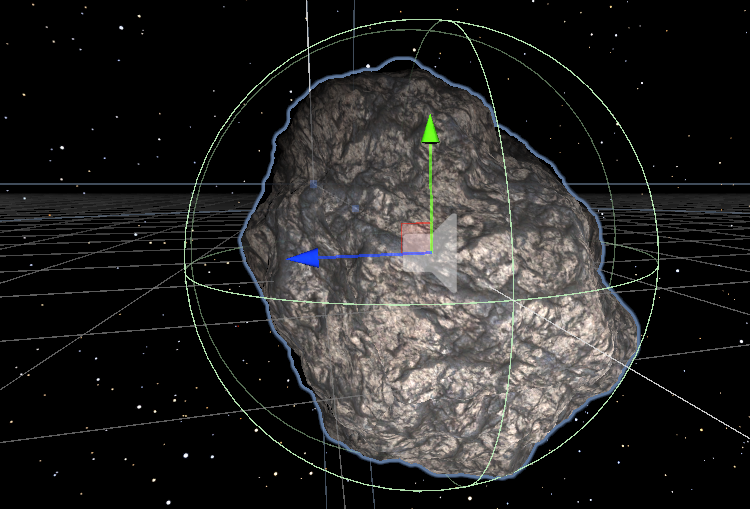
\includegraphics[scale=0.6]{hitbox.png}}
\caption{Asteroid physics proxy}
\label{fig12}
\end{figure}

A test subject reported that once he found out he intentionally aimed as far as possible from the asteroid center to be faster.\\

\subsubsection{White noise}
Three subject at the end of the test spontaneously told that white noise was easier for them to find.
One subject found our instruction not totally clear on the fact that white noise was actually a noise that gave information about asteroid position rather than some covering distracting noise. This seems to be linked to the subject previous experience with acoustics test where he was asked to hear a pitched sound while listening to white noise.\\

\subsubsection{Mono audio}
One subject told that mono audio was easier for them, also mono audio was the first test they did on the sequence. No explanation for this expect that every person is different or that he got tired while doing the others after.\\

\subsubsection{Searching pattern}
Few subject started wondering what was the best searching pattern for mono audio. The most effective one seemed to be searching horizontally while moving the mouse up and down in a sinusoidal fashion to quickly check all the elevation while moving on the azimuth. Although most subjects just searched randomly.

\section{Conclusions}
The data gathered on a total of 21 subjects shows a statistically significant difference between mono audio, stereo panning and Steam Audio HRTF. This confirms the available academic knowledge on the subject.
When analyzing the impact of different sound types, i.e. white noise, step sound and gunshot sound the data indicate that white noise performs a bit better, but the difference is not statistically significant and as such more test should be performed to confirm or deny the relevance of different sound types.
When comparing different metric, i.e. time, horizontal movement and vertical movement we show that the spatialization method influence the distance travelled more than the time. This can be useful to know as it means distance travelled is a better score indicator and could be more suited for a personal HRTF selection based on a gamification approach.
This also indicates that angular distance could be a better metric to perform future analysis on the impact of personalized HRTF on player performance.

\begin{thebibliography}{00}
\bibitem{b1} George F. Kuhn , "Model for the interaural time differences in the azimuthal plane", The Journal of the Acoustical Society of America 62, 157-167 (1977) https://doi.org/10.1121/1.381498

\bibitem{b2} S. T. Birchfield and R. Gangishetty, "Acoustic localization by interaural level difference," Proceedings. (ICASSP '05). IEEE International Conference on Acoustics, Speech, and Signal Processing, 2005., Philadelphia, PA, USA, 2005, pp. iv/1109-iv/1112 Vol. 4, doi: 10.1109/ICASSP.2005.1416207.

\bibitem{b3} Frederic L. Wightman
Department of Psychology and Waisman Center, University of Wisconsin Madison, Madison, Wisconsin 53705
Doris J. Kistler
Waisman Center, University of Wisconsin Madison, Madison, Wisconsin 53705
, "Resolution of front–back ambiguity in spatial hearing by listener and source movement", The Journal of the Acoustical Society of America 105, 2841-2853 (1999) https://doi.org/10.1121/1.426899

\bibitem{b4} M. Risoud, J.-N. Hanson, F. Gauvrit, C. Renard, P.-E. Lemesre, N.-X. Bonne, C. Vincent,
Sound source localization,
European Annals of Otorhinolaryngology, Head and Neck Diseases,
Volume 135, Issue 4,
2018,
Pages 259-264,
ISSN 1879-7296,
https://doi.org/10.1016/j.anorl.2018.04.009.

\bibitem{b5} William G. Gardner and Keith D. Martin , "HRTF measurements of a KEMAR", The Journal of the Acoustical Society of America 97, 3907-3908 (1995) https://doi.org/10.1121/1.412407

\bibitem{b6} FA. P..  Freeland, LU. P..   Biscainho, and PA. R..   Diniz, "Efficient HRTF Interpolation in 3D Moving Sound," Paper 000232, (2002 June.).

\bibitem{b7} https://valvesoftware.github.io/steam-audio/

\bibitem{b8} J. S. Andersen, R. Miccini, S. Serafin and S. Spagnol, "Evaluation of Individualized HRTFs in a 3D Shooter Game," 2021 Immersive and 3D Audio: from Architecture to Automotive (I3DA), Bologna, Italy, 2021, pp. 1-10, doi: 10.1109/I3DA48870.2021.9610934.

\bibitem{b9} https://valvesoftware.github.io/steam-audio/doc/unity/guide.html\#use-a-custom-hrtf

\bibitem{b10} Camilla H. Larsen, David S. Lauritsen, Jacob J. Larsen, Marc Pilgaard, and Jacob B. Madsen. 2013. Differences in human audio localization performance between a HRTF- and a non-HRTF audio system. In Proceedings of the 8th Audio Mostly Conference (AM '13). Association for Computing Machinery, New York, NY, USA, Article 5, 1–8. https://doi.org/10.1145/2544114.2544118

\bibitem{b11} D. Poirier-Quinot, and BR. F.. Katz, "Assessing the Impact of Head-Related Transfer Function Individualization on Task Performance: Case of a Virtual Reality Shooter Game," J. Audio Eng. Soc., vol. 68, no. 4, pp. 248-260, (2020 April.). doi: https://doi.org/10.17743/jaes.2020.0004

\bibitem{b12} D.  Poirier-Quinot, and BR. F..   Katz, "Impact of HRTF Individualization on Player Performance in a VR Shooter Game II," Paper P4-1, (2018 August.).

\bibitem{b13} Eriksson, P. R. (2017). A Comparison Of Two Commercially Available Alternatives For Spatializing Audio Over Headphones In A Game Setting.

\bibitem{b14} https://docs.scipy.org/doc/scipy/reference/generated/scipy.stats.kstest.html

\end{thebibliography}
\end{document}
    